\graphicspath{{Img/tyer/}}

\chapter{Knot tying}

    \section{Assignment} \label{sec:TheoreticalSolution}
        The work done on knot tying follows the work performed in UC Berkeley, USA. I also follow up on my own work performed in the previous semester \cite{PreDiplomaLejsekHlavac}.

        The goal is to be able to tie a simple overhand knot (see Figure~\ref{fig: over hand knot}) in the air. The procedure should be fully automated.

        \begin{figure}[h]
        \includegraphics[width=0.4\textwidth]{over_hand_knotAdj.png}
        \centering
        \caption{The over hand knot.}
        \label{fig: over hand knot}
        \end{figure}

        My working scenario is the following. The knot-tying process starts from a position when the robot holds the rope in both arms in the air. The knot is then made while still holding the rope the whole time in the air, i.e. it is not allowed to place the rope on a table. The robot thus has to release one end of the rope at a certain point of the tying process and has to ``recatch'' it again.

        To figure out the movements of the robot to tie an over hand knot, I decided to follow a human example. I simply imagined how I would tie a knot if I could only use two fingers (the gripper of the robot only has ``two fingers''). I came up with the following solution that starts from a position where the robot holds the rope in both arms.
%
        \begin{enumerate}\itemsep0pt
        \label{enu:TheoreticalSolution}
            \item Wrap the rope around the left arm in a way that a loop is created.
            \item With the right arm release the rope end and move the right arm away.
            \item Turn the left arm so that the right camera sees the loop and the rope end.
            \item Detect the rope end and catch it with the right arm.
            \item Tighten the knot using both arms.
        \end{enumerate}


    \section{Experimental setting}

        \subsection{Available Ropes} \label{sec:AvailableRopes}
            I bought six \SI{2}{m} long rope segments of different colors made from different materials (see Figure~\ref{fig:AvailableRopes}). The ropes are numbered from left to right. Table~\ref{table:AvailableRopes} shows their properties. The \emph{twisted} rope is made of a three strands, the \emph{braided} rope has a braided tubular jacket over strands of fiber and the \emph{kernmantled} rope has a kern covered with a braided tubular jacket.

            \begin{figure}
            \includegraphics[width=0.5\textwidth]{RopesAdj.png}
            \centering
            \caption{Available ropes.}
            \label{fig:AvailableRopes}
            \end{figure}

            \begin{table}\centering
            \ra{1.3}
            \begin{tabular}{@{}cccc@{}}\toprule
            Rope & color & type & diameter $\phi$ [mm]\\ \midrule
            R1 & red & twisted & 14\\
            R2 & white & twisted & 19\\
            R3 & white & braided & 19\\
            R4 & blue & kernmantled & 23\\
            R5 & blue & twisted & 26\\
            R6 & orange & flat & 1.4\\
            \end{tabular}
            \caption{Available ropes.}
            \label{table:AvailableRopes}
            \end{table}


        \subsection{Examining the Asus Kinect sensor}
            Kinect sensor provides the point cloud, i.e. the distance measurements from the observer's point of view. Kinect sends messages at an average rate of \SI{4}{Hz}. The message is an array of size 640 x 480 x 6. It resembles an image that contains information about color (RGB) and $x$, $y$ and $z$-coordinate of the given point in every pixel. Thus a depth image is obtained from the point cloud just by taking the $z$-coordinate. Furthermore, if a certain point is found in the RGB image (e.g. rope end), its coordinates in the camera coordinate system are known immediately.

    \section{Theoretical analysis}

        \subsection{Used sensors}
            To be able to follow the tying procedure (see Section~\ref{enu:TheoreticalSolution}), several sensors have to be used. In order to detect the rope end visually, the Kinect sensor is needed. To fasten the knot, the force feedback from the force/torque sensor is needed.

        \subsection{Rope requirements}
            The rope should be rather thick. Firstly, it is then easier to detect it in the depth image provided by the Kinect sensor. Secondly, it is less probable that a thicker rope gets stuck on the left arm while fastening the knot. On the other hand, the rope should not be thicker than \SI{42}{mm} which is the maximum pitch of the robot gripper.


    \section{Learning from a human example}

        \subsection{Task assignment}
            In order to test the theoretical solution proposed in Section~\ref{sec:TheoreticalSolution}, I asked two subjects (A -- sees well, B -- is blind) to tie an overhand knot on a rope. The hypothesis is that both subjects would use fingers to tie a knot at first. When only two fingers are allowed, they would come up with a similar solution as I did -- wrapping the rope around the second arm. Subject B would primarily rely on the tactile feedback to recatch the rope while subject A would primarily rely on the visual feedback. I also hypothesized that subject B would spend a lot more time analyzing the properties of the rope, e.g. its stiffness. To simulate the robotic hands even better, two scenarios will be used. In the first one, the subjects could use two fingers only and in the second one they will have to use pliers to manipulate with the rope. The following list summarizes all aforementioned scenarios.
%
            \begin{enumerate}\itemsep0pt
                \item Tie the knot as you like, i.e. you can use fingers. \label{it: fingers}
                \item Tie the knot using the pointing and the middle fingers only. \label{it: 2 fingers only}
                \item Tie the knot using pliers. \label{it: pliers}
            \end{enumerate}

        \subsection{Observing how a normally seeing and a blind person ties a knot}

            The whole experiment was recorded on a video called \textit{SubjectAB.mpg} that can be found on the attached CD.

            \paragraph{All fingers allowed, \ref{it: fingers}}~\\
                \indent Both subjects had no problems tying the knot if they could use all fingers normally. In fact, they mostly used fingers to tie the knot. Subject B was a bit slower than subject A. To fasten the knot at the end, subject B tied it in series of movements checking how tight the knot is in every step.

            \paragraph{Two fingers only, \ref{it: 2 fingers only} }~\\
                \indent Both subjects had considerable problems to tie the knot. Subject B was not able to succeed at all, while subject A came up with a very complicated solution.

                In the end, I had to change the original plan and show them my solution and asked them to repeat it. Subject A was able to follow it after I visually showed him how to do it. However, subject B had to be taught by a direct guidance, hand by hand.

                Subject B had problems making the loop around the second arm. Sometimes he created no loop at all and thus was unable to tie the knot. Even if he succeeded in making the loop, it was uneasy for him to find the rope end using only tactile feedback (see Figure~\ref{fig:SubjectAB}, the right side). He sometimes did not catch the rope end, but the loop instead. However, he was able to correctly distinguish them by trial and error.

                \begin{figure}[h]
                    \centering
                    \begin{tabular}{cc}
                    \includegraphics[height=0.3\textwidth]{ATwoFingers.png}
                    %
                    &
                    %
                    \includegraphics[height=0.3\textwidth]{BLookingForRopeEnd.png}
                    \end{tabular}
                    \caption{Left: Subject A holds the rope with two fingers. Right: Subject B caught the rope end.}
                    \label{fig:SubjectAB}
                \end{figure}

                When tightening the knot, the rope sometimes got stuck on the left arm of subject B. It required an extra effort to make the loop slide down his forearm.

            \paragraph{Pliers, \ref{it: pliers}}~\\
                \indent Subject A had no problems to tie the knot using pliers. As hypothesized, it was simple to recatch the rope.

                Subject B surprised me a lot. I hypothesized that since he had no tactile feedback from the pliers, he would be unable to tie the knot at all. However, he switched from recatching the rope end to recatching the pliers holding the rope end. He used his second arm to press the pliers against his body to prevent them from falling down (see Figure~\ref{fig:BPliers}).

                \begin{figure}[h]
                \includegraphics[width=0.7\textwidth]{BPliers.png}
                \centering
                \caption{Subject B made the knot using pliers.}
                \label{fig:BPliers}
                \end{figure}


        \subsection{Discussing the observed behavior}
            As expected, Subject A was generally faster in tying the knot than Subject B. However, subject B was able to came up with solutions that I could not imagine. It proved that subject B would not be replaceable by a normally seeing person who would only close his eyes.

            Both subjects had a lot more problems to tie the knot using two fingers only than using pliers. I think it is because of the fact that they both already worked with pliers before and thus were accustomed to using them. However, to work with two fingers only was something completely new to them.

            Subject B refrained from long and fast movements especially when tightening the knot. I think it is because he could have hit an unseen obstacle. In this way, he protected himself.

            Finally, I had to mention that the \SI{2}{m} long rope segment is well suited for the \CloPeMa\/ robot, but it is too long to be worked with for a human.


        \subsection{Implications for the robotic knot-tying}
            The \CloPeMa\/ robot is in a way similar to Subject B. Although it can use visual feedback, it is slow, because it takes a lot of time to process it.

            Based on the observation of the behavior of Subject B, I came up with the following guidelines for tying the knot programmatically.
%
            \begin{itemize}
                \item Make the loop around the left arm big enough so that there is enough space later to recognize and recatch the rope end correctly.

                \item Use visual feedback to detect the rope end as it is much faster and more reliable than the tactile feedback only.

                \item While tightening the knot, the left arm should move in a way to help the loop slide down and not get stuck.

            \end{itemize}

    \section{Finding rope end}

        \subsection{Segmentation methods}

            The main task of the knot-tying procedure is to find the previously released rope end again. I decided to use the visual information for this purpose.

            There are basically a few basic detection approaches how to segment the rope and subsequently find its end:
%
            \begin{enumerate}\itemsep0pt
                \item Background subtraction; \label{it: background subtraction}
                \item RGB based; \label{it: rgb}
                \item Depth image based. \label{it: depth}
            \end{enumerate}

            The Case \ref{it: background subtraction} requires that the background does not change while tying the knot. First, a model of the background is made from several images of the background. Only afterwards is the rope moved against it, a new image is taken and the segmentation starts. The condition that the background does not change holds in the case if the rope is wrapped around the left arm and the right one then tries to catch the rope again. However, this condition will not hold if the arms are used vice versa. In that case, the rope would hang against the safety door of the robotic cell, so there could be a change in the background when for instance a person comes in. This method was rejected because it is not general enough.

            The Case \ref{it: rgb} uses the color of the rope to segment it. However, I have a few ropes in different colors at disposal. Thus, a human would have to specify the color of the rope before the start of the knot tying. Furthermore, some ropes are white and it is obviously hard to segment such ropes against a white wall. For these reasons, this approach was rejected as well.

            Finally, the Case \ref{it: depth} uses the depth image to segment the rope. It is possible to get an estimate of how far the rope is from the camera from the positions of the arms of the robot. There are normally no other objects around this distance as no person can come close to the robot when it moves. Furthermore, the available ropes are thick enough to be seen in the depth image. For these reasons, I decided to implement rope segmentation based on the depth image.

        \subsection{Implementation of the detection algorithm}

            \begin{figure}
                \centering
                \begin{tabular}{cc}
                \includegraphics[width=0.39\textwidth]{rgb_red.png}
                %
                &
                %
                \includegraphics[width=0.39\textwidth]{depth_red.png}
                \end{tabular}
                \caption{Rope end. Left: RGB image. Right: Depth image.}
                \label{fig:RopeEndRgbAndDepth}
            \end{figure}

            The detection algorithm works with the point cloud obtained from the Kinect sensor. Figure~\ref{fig:RopeEndRgbAndDepth}, right side, shows the RGB image obtained from the point cloud and the left side shows the corresponding depth image. The images are turned almost upside down because of the position of the Kinect sensor on the right arm. I will assume the following.
%
            \begin{enumerate}\itemsep0pt
                \item There is no other object around the same distance as the rope in the image.
                \item There are always two pieces of the rope in the image: the rope loop and the rope end.
            \end{enumerate}

            The detection algorithm works with depth image only (so it does not matter which color the rope has). It also uses information from the geometry of the robot -- the distance between the origin of the camera coordinate system and the tip of the left arm called rope distance $r_d$. The rope end detection works in the following way.
%
            \begin{enumerate}\itemsep0pt
            \label{enu:RopeDetectionAlgorithm}
                \item Compute the distance $r_d$ of the rope from the camera.
                \item Segment the rope: Mark everything within $ [\left. r_{d} - 0.1, r_{d} + 0.5 \right.] $ as the rope.
                \item Find the first connected component $ C_1 $ (see Algorithm~\ref{alg:ConnectedComponents}).
                \item Find the second connected component $ C_2 $ (see Algorithm~\ref{alg:ConnectedComponents}).
                \item The smaller component (in number of pixels) is considered to be the rope end, the bigger one is considered to be the loop.
                \item Find the tip of the rope end $P_{rt}$  as the point that has the minimal $x$-coordinate index.
            \end{enumerate}

            The algorithm for finding connected components (see Algorithm~\ref{alg:ConnectedComponents}) has one important parameter -- the width $w$ [pixels]. This parameter is introduced so that the algorithm can connect pieces that are only separated by a short distance. The reason is that the depth image might not contain only two components (the rope loop and the rope end), but these components might be a bit ``scattered''. The higher the width $w$ is, the faster the algorithm is. However, there is an upper bound on $w$. The algorithm should not step over the gap between the rope loop and the rope end, i.e. it should not connect these two components into one.

            \begin{algorithm}
                \caption{Find connected components.}\label{alg:ConnectedComponents}
                \begin{algorithmic}[1]

                \Procedure{FindComponent}{maskRef, $w$}

                \State maskNew = 0 \Comment{Init maskNew - Array of the same size as maskRef}
                \State points.add($p_i$) \Comment{Randomly initialize a point.}

                \While {points.size > 0}
                    \State p = points.pop()

                    \State cut = GetArea(p, $w$, maskRef) \Comment{Select rectangular area around a point.}

                    \State maskNew[cut == 1] = 1 \Comment{Mark pixels as 1 (belonging to the component)}

                    \State pToAdd = PointsToAdd(cut) \Comment{Find 4 corner points.}

                    \While {pToAdd.size > 0}
                        pNew = pToAdd.pop()
                        \If {pNew not in pointsVisited} \Comment {Add new point if it is not already visited}
                            \State pointsVisited.add(pNew)
                            \State points.add(pNew)
                        \EndIf
                    \EndWhile

                \EndWhile

                \State \textbf{return} maskNew

                \EndProcedure
                \end{algorithmic}
            \end{algorithm}

        \subsection{Testing the detection algorithm}

            First, I analyzed the algorithm for finding connected components and experimentally estimated the parameter width $w$. The results below are from analyzing the recorded rosbag with data from working with the red rope.

            For width $w = 20$, the algorithm worked sometimes correctly, but sometimes it connected both components $C_1$ and $C_2$ into one. As there is just a little time difference for width $w=20$ and $w=15$, width was chosen to be $w=15$. Table~\ref{table:MeasuringConnectedComponents} summarizes the measured times and iterations of the algorithm. The trend in the measured times is shown graphically in Figure~\ref{fig:MeasuringConnectedComponents}.

            \begin{table}\centering
            \ra{1.3}
            \begin{tabular}{@{}ccccc@{}}\toprule
            Width $w$ [pixels] & $ t_{C_1}$ [s] & $t_{C_2}$ [s] & $i_{C_1}$ & $i_{C_1}$ \\ \midrule
            5 & 3.927 & 0.782 & 12626 & 2706 \\
            10 & 3.677 & 0.571 & 8738 & 1459 \\
            15 & 2.415 & 0.394 & 4623 & 820 \\
            20 & 2.384 & 0.410 & 3864 & 640 \\

            \bottomrule
            \end{tabular}
            \caption{Measuring Connected Components Algorithm.}
            \label{table:MeasuringConnectedComponents}
            \end{table}

            \begin{figure}
            \includegraphics[width=0.5\textwidth]{MeasuringConnectedComponents.png}
            \centering
            \caption{Measuring Connected Components Algorithm.}
            \label{fig:MeasuringConnectedComponents}
            \end{figure}



        \subsection{Experimental results}

            Figure~\ref{fig:RopeEndDetection} shows the results of the detection algorithm. The first image shows the segmentation of the rope in the depth image based on the guessed rope distance $d_r$. The second image shows the first connected component $C_1$ and the third image shows the second connected component $C_2$. In our case, $C_1$ is bigger in size (the amount of pixels) than~$C_2$, so~$C_1$ is considered to be the rope loop and $C_2$ the rope end. The tip of the rope end $P_{rt}$ is denoted by a green dot in the fourth image.

            \begin{figure}
                \centering
                \begin{tabular}{cc}
                \includegraphics[width=0.39\textwidth]{RopeSegmentationAdj.png}
                %
                &
                %
                \includegraphics[width=0.39\textwidth]{RopeLoopAdj.png}
                \\
                1 & 2 \\
                \includegraphics[width=0.39\textwidth]{RopeEndAdj.png}
                %
                &
                %
                \includegraphics[width=0.39\textwidth]{RopeEndDetectedAdj.png} \\
                3 & 4 \\

                \end{tabular}
                \caption{1: Rope segmentation, 2: $C_1$ rope loop, 3: $C_2$ rope end, 4: Rope tip $P_{rt}$ detected.}
                \label{fig:RopeEndDetection}
            \end{figure}


    \section{Knot-tying procedure}


        Based on the theoretical analysis, a work flow of the knot-tying procedure was designed (see Figure~\ref{fig:TyerWorkflow}). Below is a more detailed description of the states of the knot-tying procedure. A diagram connected with each state is shown in Figure~\ref{fig:TyerStates} and Figure~\ref{fig:TyerTighten}.

        \begin{figure}
        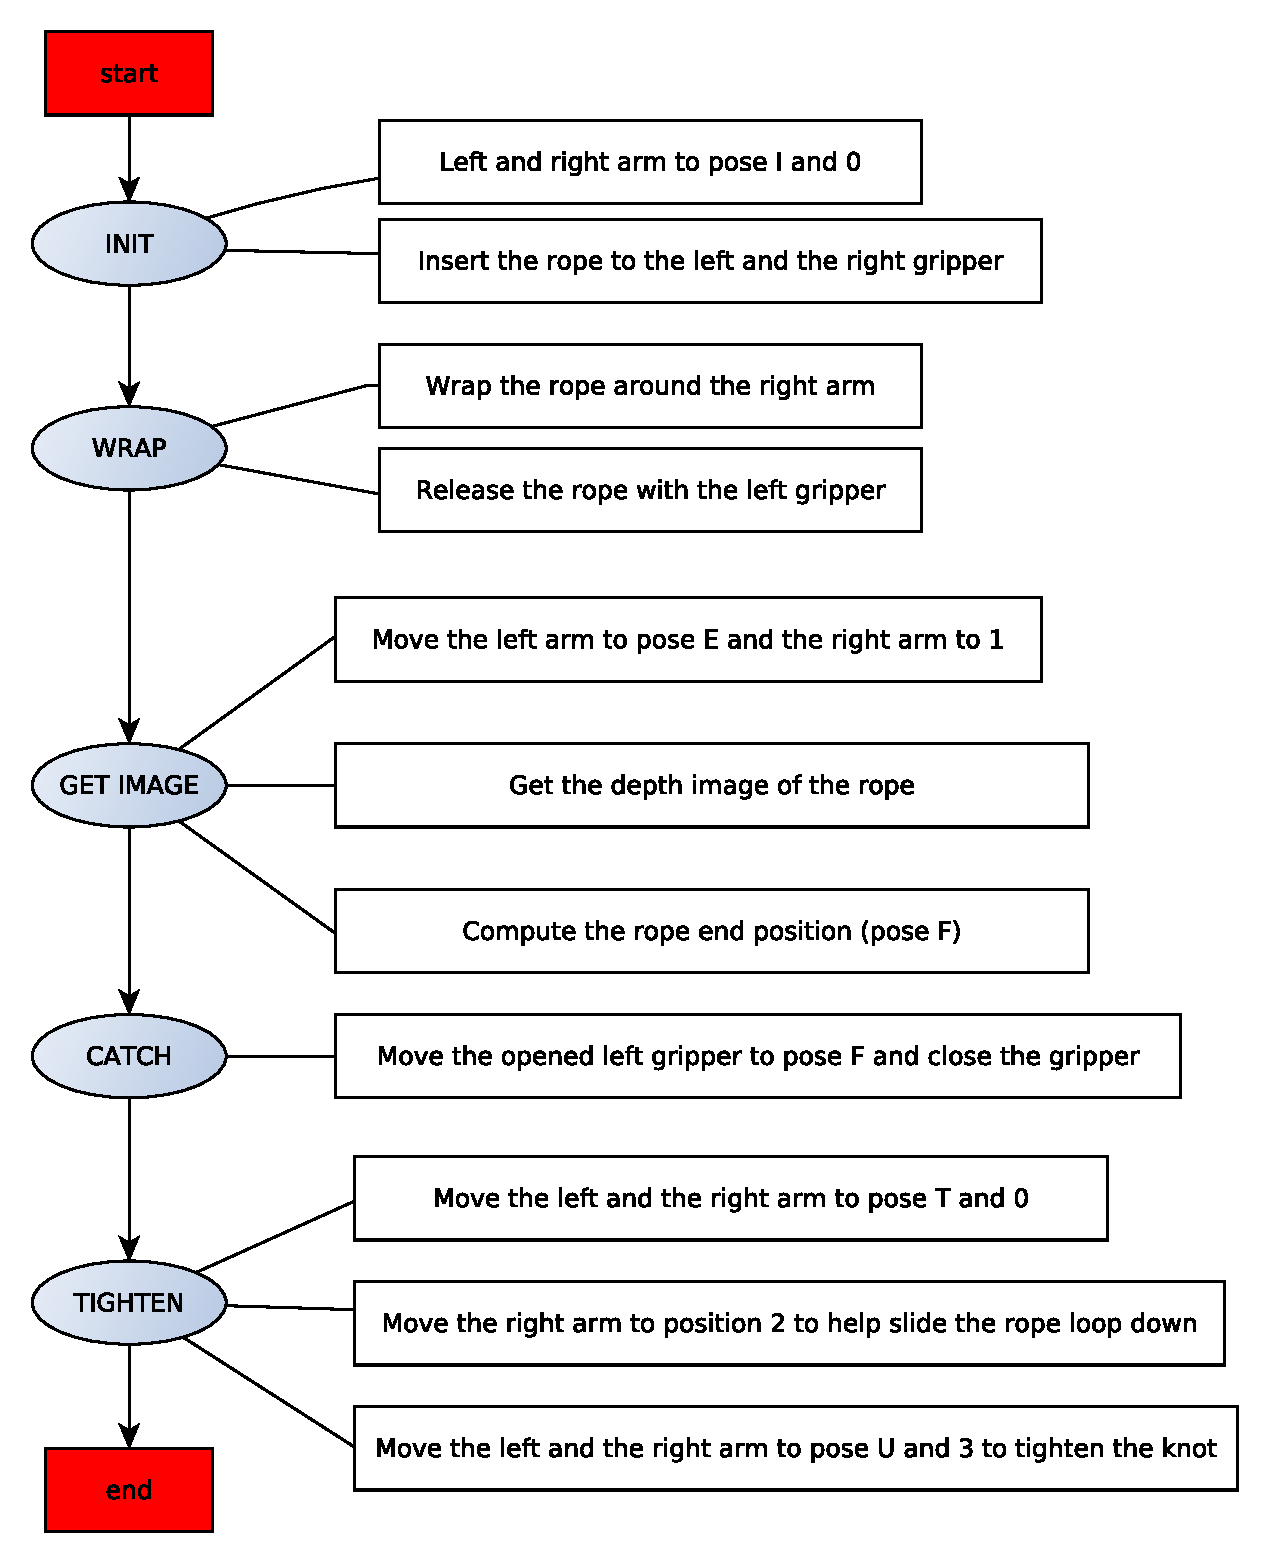
\includegraphics[width=0.8\textwidth]{TyerWorkflow.pdf}
        \centering
        \caption{Knot-tying work-flow.}
        \label{fig:TyerWorkflow}
        \end{figure}

        \begin{figure}
            \centering
            \begin{tabular}{c|c}
            \includegraphics[width=0.4\textwidth]{01Init.png}
            &
            \includegraphics[width=0.4\textwidth]{02Wrap.png} \\
            1 & 2 \\
            \hline
            \includegraphics[width=0.4\textwidth]{03GetImage.png}
            &
            \includegraphics[width=0.4\textwidth]{04Catch.png} \\
            3 & 4 \\

            \end{tabular}
            \caption{1: INIT, 2: WRAP, 3: GET IMAGE, 4: CATCH.}
            \label{fig:TyerStates}
        \end{figure}


        \begin{figure}
        \includegraphics[width=0.6\textwidth]{05Tighten.png}
        \centering
        \caption{TIGHTEN.}
        \label{fig:TyerTighten}
        \end{figure}



        \paragraph{INIT}~\\
        \noindent The tying procedure starts with the two grippers facing each other, right in pose $P_I$ and left in $P_0$ (see Figure~\ref{fig:TyerStates} - 1). Both grippers hold the ends of the rope.

        \paragraph{WRAP}~\\
        \noindent The right arm goes through poses $P_A$, $P_B$, $P_C$ and $P_D$ (see Figure~\ref{fig:TyerStates} - 2). The rope thus forms a loop around the left arm. Finally, the right gripper releases the rope end.

        \paragraph{CAPTURING THE IMAGE}~\\
        First, the left arm turns to pose $P_1$ to enable catching the rope end later. Second, the right arm moves to pose $P_E$ in order to have a good view of the rope loop and the rope end hanging on the left arm (see Figure~\ref{fig:TyerStates} - 3). Third, the right gripper closes and moves to get out of sight. The point cloud from the Kinect sensor is captured. Finally, the rope end is detected from the depth image. Pose of the rope end $P_F$ is computed.

        \paragraph{CATCH}~\\
        \noindent  The right gripper opens, the right arm moves to pose $P_F$ to catch the rope end. The gripper closes again. Next, the right arm moves back out of the loop to pose $P_G$ (see Figure~\ref{fig:TyerStates} - 4).

        \paragraph{TIGHTEN}~\\
        \noindent After the rope end is caught, both arms move to poses $P_T$ and $P_0$. The left arm then moves to pose $P_2$ to help the rope loop slide down of the robot arm . Finally, both arms start slowly moving from each other to poses $P_U$ and $P_3$ (see Figure~\ref{fig:TyerTighten}). The magnitude of the $z$-coordinate of the force from the right force sensor $F_z$ is measured. If the measured force exceeds the experimentally estimated threshold $F_{thresh} = \SI{10}{N}$ (meaning that the knot is already tightened), the motion of both arms is stopped.


    \section{Experiments}
        I tested the developed knot-tying script on ropes R1-5 (see Table~\ref{table:AvailableRopes}). Since R6 is flat and thus it is hard to detect it in the depth image, it was omitted from the experiments.

        I also changed the width parameter $w$ to 10. I did it due to further experiments with the red rope. Sometimes the rope end and rope loop were very close to each other. If $w=15$, both connected components merged into one and the rope end detection was not possible.

       The observations are listed below:
%
        \begin{itemize}\itemsep 0pt
            \item The proposed solution was successful in the case of R1 and R4 (successful rope end detection in Figure~\ref{fig:R4success}). It took around $65$ seconds to tie the knot (see video \textit{KnotTying.mpg} that can be found on the attached CD). Figure~\ref{fig:R1R4KnotTightening}, left side shows the knot tying process of R1 and Figure~\ref{fig:R1R4KnotTightening}, right side shows the successfully made knot on the rope R4.

            \begin{figure}
                \centering
                \begin{tabular}{cc}
                \includegraphics[height=0.3\textwidth]{R1KnotTightening.png}
                &
                \includegraphics[height=0.3\textwidth]{R4KnotTightening.png}

                \end{tabular}
                \caption{Left: Tightening the knot on the rope R1, Right: The knot made on the rope R4.}
                \label{fig:R1R4KnotTightening}
            \end{figure}

            \item The rope end was sometimes not found correctly in the case of R2 and R3 (see Figure~\ref{fig:R2R3failure}).
            \item R5 got stuck on the left arm during tightening.
        \end{itemize}


        \begin{figure}
            \centering
            \begin{tabular}{cc}
            \includegraphics[width=0.39\textwidth]{R4SegmentationAdj.png}
            &
            \includegraphics[width=0.39\textwidth]{R4RopeEndFoundAdj.png}

            \end{tabular}
            \caption{Left: R4 segmentation, Right: R4 rope end found.}
            \label{fig:R4success}
        \end{figure}

        \begin{figure}
            \centering
            \begin{tabular}{cc}
            \includegraphics[width=0.39\textwidth]{R2SegmentationAdj.png}
            &
            \includegraphics[width=0.39\textwidth]{R3SegmentationAdj.png}


            \end{tabular}
            \caption{Left: R2 segmentation, Right: R3 segmentation.}
            \label{fig:R2R3failure}
        \end{figure}

    \section{Discussion}
        It turned out that the proposed solution is mainly successful for non-white and non-twisted ropes. The rope should not be flat, but should also not be thicker than the gripper pitch.

        If the rope is white, the obtained segmentation in the depth image has huge gaps between the many connected components (see Figure~\ref{fig:R2R3failure}). Thus, the precondition that the segmentation should contain only two connected components is violated and the rope end detection fails.

        The twisted ropes not only cause the same problems during rope end detection as the white ones, but they also tend to get stuck on the robot arm.

        The mentioned issues relate to image segmentation. I used a simple segmentation algorithm because the image segmentation is an unsolved problem. Image segmentation is the object of the intensive research by others.

